\chapter{实数}\label{chp:real}
实数是现实世界中最基本的数系,我们采用逼近法来研究实数,逼近法是一种原理简朴但是应用广泛的方法,它将贯穿于本书的微积分学部分,是一支主力军。

\section{度量与实数}

一般说来,常见的量可以归纳成两类:比如一堆蛋,一群牛,它们都具有天然的个别单元,对它们的处理方法是数一数它们的个数,用来数个数的数学体系就是“自然数系”。另一类量如长度、重量、温度、压力这种量不具有天然不可分割的单元!我们处理这类量的办法是度量,由度量产生的数系就是“实数系”,换句话说,实数系乃是将常见的长度、重量等这一类量的通性加以抽象化、组织化所得出来的数学体系,它是用来表达、计算这一类连续变化的量的简洁、有效工具。

下面将以长度为例,说明度量和实数的起源。

\subsection{长度的度量}
因为长度这种量并不是有天然不可分割的单位,所以我们只好选用人为的单位长,设线段 $u$ 是所选用的单位长,当我们要度量一个线段 $a$ 时,我们所要去求的乃是 $a$ 与 $u$ 之间的“比值”,这个比值是一个实数 $k$, 我们就说线段 $a$ 的长度是 $k$ 单位,现在让我们耐心地分析一下,在实践中这个“比值”是怎样求得的?

我们先拿一根尺 $u$, 用它去逐段比量线段 $a$, 假如 $a$ 恰好是 $n$ 个和 $u$ 等长的线段首尾连接而成,我们说 $u$ 恰好整量 $a$, $a$ 的长度是 $n$ 单位,但是假如 $u$  不能整量 $a$,例如在\cref{fig:segments} 中的线段,$a$ 比 $4u$ 要长些,却比 $5u$ 要短些。

\begin{figure}
\begin{tikzpicture}
\draw (0,1)--node[above]{$u$}(1,1);
\foreach \x in {0,1}
{
    \draw (\x,1)--(\x,1.1);
}
\draw (0,0)--node[above=5pt]{$a$}(4.75,0);
\foreach \x in {0,1,...,4,4.25,4.5,4.75}
{
    \draw (\x,0)--(\x,0.1);
}
\end{tikzpicture}
    \caption{}\label{fig:segments}
\end{figure}

{
\linespread{1.6}\selectfont
试着去解决上述不能整量的矛盾的一个简朴想法是:把单位长 $u$ 适当地加以等分,希望分后的“分单位”能够整量 $a$(比如上面的例子中,$\dfrac{1}{4}u$ 就可以整量 $a$, 即 $a=4\dfrac{3}{4}u=\dfrac{19}{4}u$),一般地,假如 $a$ 能用 $\dfrac{1}{m}u$ 这个分单位整量,譬如 $a=\dfrac{n}{m}u$,则 $a,u$ 之间的比值是个有理数(也称为比数)。在这儿,就自然地产生下述基本问题。\par}

\bigskip
\emph{度量基本问题 } 任给两个量 $a,b$ 之间的比值是否一定是个有理数(比数)?换句话说,对于任给两个量 $a,b$ 是否存在一个同时整量 $a,b$ 的 $u$?

上面这个问题的重要性可以分别从正、反两面来分析:假如任何两个量的比值总是有理数,那么有理数全体就足够处理度量问题,这样度量问题就变得十分简单了。从另一方面来看,假如两个量之间的比值不一定是有理数,则有理数全体(简称有理数系或比数系)就不足以处理度量问题,换句话说,我们就得学会一个不只包含有理数系的实数系,才能充分处理度量问题。总之,上述基本问题是必须实事求是地弄明白的!

\subsection{无理数(非比实数)的存在}
不难给出,两个线段的比值不可能是有理数的一个简单例子,如\cref{fig:irrationalnumber} 所示,各边为单位长度的正方形的对角线 $\ell$ 与边长之比就不能是个有理数。
\begin{figure}
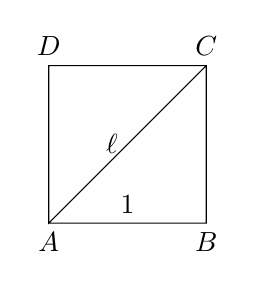
\begin{tikzpicture}
\draw (0,0)node[below]{$A$} --node[above]{1}(2,0)node[below]{$B$}-- (2,2)node[above]{$C$}--(0,2)node[above]{$D$}--(0,0)--node[left]{$\ell$}(2,2);
\end{tikzpicture}
\caption{}\label{fig:irrationalnumber}
\end{figure}

因为根据勾股定理,$\ell^2=2$, 所以,如果 $\ell$ 是个有理数,设其等于 $\dfrac{p}{q}$,这里 $q$ 和 $p$ 是两个互质的正整数,我们将有
\[p^2=2q^2\]
根据上述方程,$p$ 是偶数,因此 $p$ 本身也必定是偶数,譬如说,$p=2p'$, 用 $2p'$ 代替 $p$, 我们得到
\[4({p'}^2)=2q^2\]
或者,
\[q^2=2(p')^2\]
{\linespread{1.6}\selectfont
因而 $q^2$ 是偶数,于是 $q$ 也是偶数,然而这同我们所作的 $p$ 和 $q$ 没有公因子的约定相矛盾,这一矛盾是由假设对角线长能够表示为既约分数 $\dfrac{p}{q}$ 引起的,所以这一假设是错误的。\par}

这一用反证法推导的例子,表明符号 $\sqrt{2}$ 不能对应于任何有理数。另一例子是$\uppi$ ——圆的周长与直径的比,证明 $\uppi$ 不是有理数要复杂得多,并且直到近代才做到。不属于有理数系的实数有很多,所以在某种意义上远比有理数更为普遍,因此,从几何度量的客观实际需要出发,我们不得不增添一类新数,这一类新数叫\emph{无理数}。有理数和无理数的全体统称为\emph{实数系}。当我们面对着实数系中还存在着许多“无理数”这一事实时,怎样去有系统地学习实数系的性质并充分掌握其用法,这便成为我们的一个迫切的基本课题。下面所要谈的逼近法,就是一种有效地利用熟知的有理数系作为桥梁,向实数系进军的捷径。

\subsection{逼近法}
通过已知的有理数系去了解实数系的可能性基于下述基本事实,那就是:任何无理数都可以用有理数去逼近它!现在我们用数轴来图解有理数系与实数系间的关系。如\cref{fig:approximation} 所示。

\begin{figure}
\begin{tikzpicture}[>=latex, scale=1.3]
\draw[very thick, ->] (-0.8,0)--(8,0)node[right]{$\ell$};
\foreach \x/\xtext in {0/0,1/\dfrac{1}{q},2/\dfrac{2}{q},5.5/\dfrac{p}{q},6.5/\dfrac{p+1}{q}}
{
    \draw (\x, 0)node[below]{$\xtext$}--(\x,.1);
} 
\draw (5.9,0)--(5.9,.1)node[above]{$x$};
\end{tikzpicture}
    \caption{}\label{fig:approximation}
\end{figure}

{\linespread{1.6}\selectfont
在上面坐标系中,所有以整数为坐标的点,在直线 $\ell$ 上成一均匀分布的点集,其相邻两点间的距离都是 1 单位;同样的,所有坐标是 $\dfrac{p}{2}$, $(p=0,\pm1,\pm2,\ldots)$ 的点,在直线上成一均匀分布的点集,其相邻两点间的距离都是 $\dfrac{1}{2}$ 单位;设$q$为一指定的自然数,则所有坐标是 $\dfrac{p}{q},\; p\in\mathbb{Z}$ 的点在直线上成一均匀分布的点集,其相邻两点间的距离是 $\dfrac{1}{q}$ 单位。只要将 $q$ 取成足够大的自然数,则能使数 $\dfrac{1}{q}$ 想要多么小就可以多么小。这个现象说明在直线上任何一段很短的线段中,都有坐标是有理数的点,也就是任何两个有理数点之间都有有理数点,这就是\emph{有理数点集稠密性},但是这个现象并不表示有理点就可以填满整个直线,例如长度为 $\sqrt{2}$, $\sqrt{3}$ 的线段,若将它的一个端点放在数轴的原点,则另一端点在直线的坐标就不是有理数。现在我们的问题是如何说明实数同原来熟悉的有理数,因而最终同整数的关系。让我们再回到\cref{fig:approximation} 的数轴 $\ell$上,显然 $\ell$ 上面的每一个点或者是坐标为 $\dfrac{p}{q}$ 的有理点,或者处于两个相邻的有理点 $\dfrac{p}{q}$和$\dfrac{p+1}{q}$ 之间,换言之,给了任何自然数 $q$ 之后,对于每一个实数 $x$, 一定有一整数  $p$, 使得\par}
\[\frac{p}{q}\leqslant x<\frac{p+1}{q}\]
即
\[\frac{p}{q}\leqslant x<\frac{p}{q}+\frac{1}{q}\]
从这三个数各减去 $\dfrac{p}{q}$,得到
\[0\leqslant x-\frac{p}{q}<\frac{1}{q}\]
于是
\[\left|x-\frac{p}{q}\right|<\frac{1}{q}\]
这个不等式说明,只要将 $q$ 取成足够大的自然数,每一个实数 $x$ 与有理数 $\dfrac{p}{q}$ 的误差想要多么小就可以多么小。

下面我们来说明每一个无理数如何通过越来越逼近它的有理数数列来描述它。

\subsubsection{二分逼近法}

现在让我们用二分逼近法来说明任何无理数都可以用有理数数列去逼近它,使得误差小到任意小。

设某无理数 $x$ 位于线段 $A_0B_0=[a_0,b_0]$ 内(亦即$a_0<x<b_0$,$a_0$,$b_0$ 均为有理数),见\cref{fig:rationalnumber}。

\begin{figure}
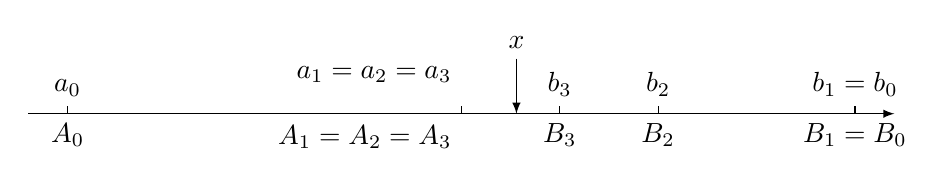
\begin{tikzpicture}[>=latex]
\draw[->] (-0.5,0)--(10.5,0);
\foreach \x/\xtext in {0/a_0,10/b_1=b_0,7.5/b_2,6.25/b_3}
{
    \draw (\x,0)--(\x,.1)node[above]{$\xtext$};
}  
\draw (5,0)--(5,.1);

\node at  (5,-.3)[left]{$A_1=A_2=A_3$};
\node at (6.25,0)[below]{$B_3$};
\node at (7.5,0)[below]{$B_2$};
\node at (0,0)[below]{$A_0$};
\node at (10,0)[below]{$B_1=B_0$};
\node at  (5,.5)[left]{$a_1=a_2=a_3$};
\draw[->] (5.7,.7)node[above]{$x$}--(5.7,0);
\end{tikzpicture}   
    \caption{}\label{fig:rationalnumber}
\end{figure}

{\linespread{1.6}\selectfont 我们将线段 $A_0B_0=[a_0,b_0]$ 等分为两段,亦即 $\left[a_0,\dfrac{a_0+b_0}{2}\right]$ 和 $\left[\dfrac{a_0+b_0}{2},b_0\right]$;而把 $x$ 所在的那一段叫做 $A_1B_1=[a_1,b_1]$,换句话说,当 $a_0<x<\dfrac{a_0+b_0}{2}$ 时,$a_1=a_0$,$b_1=\frac{a_0+b_0}{2}$;当 $\dfrac{a_0+b_0}{2}<x<b_0$,$a_1=\dfrac{a_0+b_0}{2}$,$b_1=b_0$。这样逐次二等分,由 $A_1B_1$ 求得 $A_2B_2$,\ldots,由 $A_{n-1}B_{n-1}$ 求得 $A_nB_n$,永远无休止地二等分下去,因为每次二等分后,分段长度减半,所以 $x$ 所在的线段就可以小到任何需要的程度。现在把上面的二分逼近过程写下来,就得到 $a_n,b_n,x$ 的下列关系:\par}
\begin{enumerate}
    \item $A_0B_0=[a_0, b_0]\supseteq A_1B_1 =[a_1,b_1]
    \supseteq \cdots \supseteq A_nB_n=[a_n, b_n]\supseteq A_{n+1}B_{n+1}=[a_{n+1},b_{n+1}]\supseteq \cdots \supseteq \{x\}$,即:
\[a_0\leqslant a_1\leqslant a_2\le\cdots\leqslant a_n\leqslant \cdots <x<\cdots\leqslant b_n\le\cdots\leqslant b_2\leqslant b_1\leqslant b_0\]

\item {\linespread{1.6}\selectfont $b_n-a_n=\dfrac{1}{2}(b_{n-1}-a_{n-1})=\cdots=\dfrac{1}{2^n}(b_0-a_0)$,这就保证了 $a_n$ 或 $b_n$ 和 $x$ 之间的误差小于 $\dfrac{1}{2^n}(b_0-a_0)$, 即 $|x-a_n|<\dfrac{1}{2^n}(b_0-a_0)$ 或 $|x-b_n|<\dfrac{1}{2^n}(b_0-a_0)$, 只要 $n$ 够大,上述误差就可以小到任意小。\par}
\item 实数 $x$ 由它的夹逼数列:
\[a_0\leqslant a_1\leqslant a_2\le\cdots\leqslant a_n\leqslant \cdots <x<\cdots\leqslant b_n\le\cdots\leqslant b_2\leqslant b_1\leqslant b_0\]
其中:$b_n-a_n=\dfrac{1}{2^n}(b_0-a_0)$ 唯一确定,即没有另一点能够处在所有的线段 $A_nB_n$ 之中。
\end{enumerate}

要证明这个数的唯一性,我们假定另有第二个数 $y$ 也属于一切线段 $A_nB_n$ 之中,于是这些线段的每一个长 $b_n-a_n$ 都应不小于 $|x-y|$, 但是,因为线段 $A_nB_n$ 可以任意小,只要 $n$ 足够大,$A_nB_n$ 的长就会小于 $x$ 和 $y$ 之间的距离,这就得出矛盾。所以实数 $x$ 能由它的夹逼数列唯一确定。

现在以 $x=\sqrt{2}$, $a_0=1$, $b_0=2$ 为例来说明如何用二分逼近法求 $\sqrt{2}$ 的近似值,如\cref{fig:sqrt2} 所示。
\begin{figure}
\begin{tikzpicture}[>=latex]
    \draw[->] (-0.5,0)--(10.5,0);
\foreach \x /\xtext in {0/a_0=a_1=1,10/b_0=2,5/{},2.5/a_2,3.75/a_3=a_4, 4.375/{}}
{
    \draw(\x,0)--(\x,.1)node[above]{$\xtext$};
}

\draw[->] (4.14,-.7)node[below]{$\sqrt{2}$}--(4.14,0);

\node at (5,-0.3)[right]{$b_1=b_2=b_3$};
\node at (4.375,-0.3){$b_4$};
\end{tikzpicture}
    \caption{}\label{fig:sqrt2}
\end{figure}

\begin{enumerate}
    \item  $\dfrac{1}{2}\left(a_{0}+b_{0}\right)=\dfrac{3}{2},\qquad \left(-\dfrac{3}{2}\right)^{2}=\dfrac{9}{4}>2 \quad\Rightarrow\quad\dfrac{3}{2}>\sqrt{2}$,
    
    故 $a_{0}=a_{1}=1,\qquad   b_{1}=\dfrac{3}{2}$

    \item   $\dfrac{1}{2}\left(a_{1}+b_{1}\right)=\dfrac{5}{4},\qquad \left(\dfrac{5}{4}\right)^{2}=\dfrac{25}{16}<2 \quad\Rightarrow\quad \dfrac{5}{4}<\sqrt{2}$
    
    故 $a_{2}=\dfrac{5}{4}, \qquad  b_{2}=b_{1}=\dfrac{3}{2}$

    \item  $\dfrac{1}{2}\left(a_{2}+b_{2}\right)=\dfrac{11}{8},\qquad \left(\dfrac{11}{8}\right)^{2}=\dfrac{121}{64}<2 \quad\Rightarrow\quad \dfrac{11}{8}<\sqrt{2}$
    
    故 $a_{3}=\dfrac{11}{8},\qquad  b_{3}=b_{2}=\dfrac{3}{2}$

    \item   $\dfrac{1}{2}\left(a_{3}+b_{3}\right)=\dfrac{23}{16},\qquad \left(\dfrac{23}{16}\right)^{2}=\dfrac{529}{256}>2 \quad\Rightarrow\quad \dfrac{23}{16}>\sqrt{2}$
    
    故 $a_{4}=a_{3}=\dfrac{11}{8},\qquad  b_{4}=\dfrac{23}{16}$

    \item  $\dfrac{1}{2}\left(a_{4}+b_{4}\right)=\dfrac{45}{32},\quad \left(\dfrac{45}{32}\right)^{2}=\dfrac{2025}{1024}<2 \quad\Rightarrow\quad \dfrac{45}{32}<\sqrt{2}$
    
     故 $a_{5}=\dfrac{45}{32}, \qquad b_{5}=b_{4}=\dfrac{23}{16}
    $
    
    \item  $\dfrac{1}{2}\left(a_{5}+b_{5}\right)=\dfrac{91}{64},\quad \left(\dfrac{91}{64}\right)^{2}=\dfrac{8281}{4096}>2 \quad\Rightarrow\quad \dfrac{91}{64}>\sqrt{2}$
    
     故 $a_{6}=a_{5}=\dfrac{45}{32}, \qquad b_{6}=\dfrac{91}{64}$

    
    \item  $\dfrac{1}{2}\left(a_{6}+b_{6}\right)=\dfrac{181}{128},\quad \left(\dfrac{181}{128}\right)^{2}=\dfrac{32761}{16314}<2 \quad\Rightarrow\quad \dfrac{181}{128}<\sqrt{2}$
    
    {\linespread{1.9}\selectfont 故 $a_{7}=\dfrac{181}{128}, \qquad b_{7}=b_{6}=\dfrac{91}{64}$,这时,$\dfrac{181}{128}<\sqrt{2}<\dfrac{91}{64}$,把 $\dfrac{181}{128}$ 作为 $\sqrt{2}$ 的不足近似值,其误差小于 $\dfrac{1}{2^7}=\dfrac{1}{128}$。\par}
\end{enumerate}

\medskip
{\linespread{1.6}\selectfont 照这样逐步计算,每次只要检验 $\dfrac{1}{2}(a_{n-1}+b_{n-1})$ 的平方和 2 之间的大小次序关系,就能确定 $\dfrac{1}{2}(a_{n-1}+b_{n-1})$ 应该是 $a_n$ 还是 $b_n$, 显然的,这样所求得的 $a_n,b_n$ 和 $\sqrt{2}$ 有下列关系:\par}
\[a_n<\sqrt{2}<b_n,\quad b_n-a_n=\frac{1}{2^n},\; (n=1,2,3,\ldots)\]

我们可以把 $a_n$ 叫做 $\sqrt{2}$ 的一个“$n$ 阶不足近似值”。$b_n$ 叫做 $\sqrt{2}$ 的一个“$n$ 阶过剩近似值”,它们和 $\sqrt{2}$ 的差的绝对值小于 $\dfrac{1}{2^n}$。


\subsubsection{十分逼近法}

上面所讨论的二分逼近法只不过是逼近法的一种,譬如,对于任何大于 1 的整数 $q$, 我们可以仿照上法用逐次 $q$ 等分而得到“ $q$ 分逼近法”,但是实用起来,$q$ 愈大则每次要去确定 $x$ 属于 $q$ 个分段中的哪一段时所需做计算也就愈繁,所以二分逼近法比较简便,再者,在 $q$ 分逼近法中,用来逼近的数 $a_n,b_n$ 都是那些分母是 $q$ 的方幂的分数;而常用的“十进小数”也就是分母是 10 的方幂的分数,例如,
\[1.4=\frac{14}{10},\quad  1.41=\frac{141}{100}=\frac{141}{10^2},\quad \ldots \]
所以十分逼近法也就是用小数去逼近的方法,现在再以 $\sqrt{2}$ 为例,简要地说明十分逼近法如下:

将线段 $[1,2]$ 十等分,其分点分别是 $1.1,1.2,\ldots,1.9$, 看看哪些分点的平方小于 2, 哪些大于 2,算一下就得出:

$(1.1)^2,(1.2)^2,(1.3)^2,(1.4)^2=1.96<2<2.25=(1.5)^2,(1.6)^2,\ldots ,(1.9)^2$。所以 $1.4<\sqrt{2}<1.5$,$\sqrt{2}$ 属于分段 $[1.4,1.5]$;

再把 $[1.4,1.5]$ 十等分,分点分别是 $1.41,1.42,\ldots,1.49$,再算一下,由$(1.41)^2=1.9891<2<2.0164=(1.42)^2,(1.43)^2,\ldots,(1.49)^2$,就得出 $\sqrt{2}$ 属于分段 $[1.41,1.42]$,再一次十等分,然后再由计算可以确定 $\sqrt{2}$ 属于分段  $[1.414,1.415]$,这样逐次十等分,就可以求得一个 $n$ 位小数 $a_n$ 使得
\[a_n<\sqrt{2}<b_n=a_n+\left(\frac{1}{10}\right)^n\]

在实用时,我们按照实际问题所需要的精确度,求到足够位数(即 $\left(\frac{1}{10}\right)^n$ 小于许可误差)。这里我们用普通的算术法则对 2 作开方运算将得到一个足够精确的小数。例如,求 $\sqrt{2}$ 的不足近似值和过剩近似值,精确到 $\dfrac{1}{10^4}$。计算如下:

\begin{center}
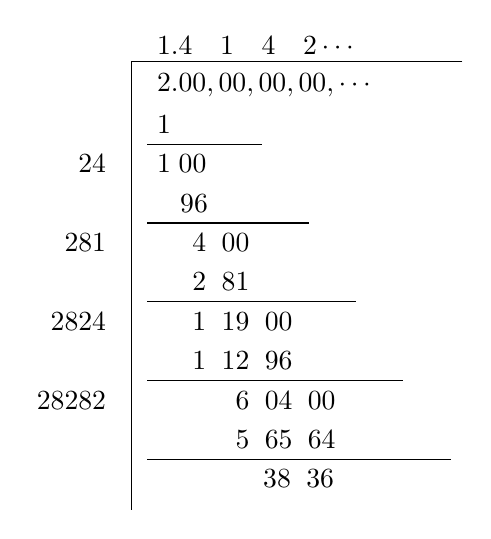
\begin{tikzpicture}[scale=2]
\node at (0,0)[right]{$\qquad \quad\;\;\;  38\;\;36$};
\node at (0,0.25)[right]{$\qquad\;\;\;  5\;\;65\;\;64$};
\node at (0,0.5)[right]{$\qquad \;\;\; 6\;\;04\;\;00$};
\node at (0,0.75)[right]{$\quad \; 1\;\;12\;\;96$};
\node at (0,1)[right]{$\quad \; 1\;\;19\;\;00$};
\node at (0,1.25)[right]{$\quad\; 2\;\;81$};
\node at (0,1.5)[right]{$\quad \; 4\;\;00$};
\node at (0,1.75)[right]{$\;\;\; 96$};
\node at (0,2)[right]{$1\;00$};
\node at (0,2.25)[right]{$1$};
\node at (0,2.5)[right]{$2.00,00,00,00,\cdots$};
\node at (0,2.75)[right]{$1.4\quad1\quad4\quad2\cdots$};
\draw(2,2.65)--(-0.1,2.65)--(-0.1,-.2);

\foreach \x/\xtext in {2/24,1.5/281,1/2824,.5/28282}
{
   \node at (-.2,\x)[left]{\xtext};
}

\foreach \x in {2.125,1.625,...,0.125}
{
    \draw (0,\x)--(2-.6*\x,\x);
}
\end{tikzpicture}
\end{center}

从计算中知道
\[1.4142<\sqrt{2}<1.4143\]
\[|\sqrt{2}-1.4142|<\frac{1}{10^4}, \qquad |\sqrt{2}-1.4143|<\frac{1}{10^4}\]

因此,1.4142, 1.4143 分别是 $\sqrt{2}$ 的精确到 $\dfrac{1}{10^4}$ 的不足近似值与过剩近似值。

\medskip
总结上面对于逼近法的讨论,我们得到了下列几点简要的初步认识:
\begin{enumerate}
    \item 实数系,有理数系,整数系,自然数系的包含关系是这样的:
\[\begin{split}
    &\qquad \mathbb{R}\quad \supset \quad \mathbb{Q}\quad \supset \quad \mathbb{Z}\quad \supset \quad \mathbb{N}\\
    &\text{实数系\quad 有理数系\quad 整数系\quad 自然数系}
\end{split}
\]

实数系还包括无理数,任何无理数都可以用有理数去逼近它!二分逼近法和 $q$ 分逼近法是各种逼近法中最常用的几种。
\item 一般说来,逼近法就是对于某一给定实数 $x$ 逐步地去求它的近似值 $a_n$,使得误差 $|x-a_n|$ 可以小到任意小。在 $q$ 分法中,使得误差小到任意小的办法是用逐次$q$ 等分同时求出一个“不足近似值” $a_n$ 和一个“过剩近似值” $b_n$,它们把所要逼近的实数 $x$ 夹逼在当中,即 $a_n<x<b_n$。因为当 $n$ 逐步增大时,$b_n-a_n=\dfrac{b_0-a_0}{q^n}$ 是显然可以小到任意小!这也就是说,给定实数 $x$ 由它的不足近似值数列 $\{a_1,a_2,\ldots ,a_n,\ldots\}$ 和过剩近似值数列 $\{b_1,b_2,b_3,\ldots ,b_n,\ldots \}$ 唯一确定。

\item 更普遍地,对给定的实数 $x$, 用某种方法得到两
个无穷数列 $\{a_1,a_2,\ldots ,a_n,\ldots\}$ 和 $\{b_1,b_2,\ldots ,b_n,\ldots \}$, 它们和 $x$ 之间满足下列关系:
\[a_1\leqslant a_2\leqslant \cdots \leqslant a_n\leqslant \cdots<x<\cdots\leqslant b_n\leqslant \cdots\leqslant b_2\leqslant b_1\]
而且在 $n$ 不断增大时,$(b_n-a_n)$ 可以小到任意小,则 $\{a_n\}$ 就叫做 $x$ 的一个“左逼近数列”,$\{b_n\}$ 就叫做 $x$ 的一个“右逼近数列”,它们分别从左、右夹逼 $x$,这样,$x$ 也就由这两组数列唯一确定。
\end{enumerate}


\subsection{实数系的基本性质}
实数系是计算长度、面积、重量、时间等等这一类量不可缺少的工具。实数系具有四则运和大小次序这两种基本结构。现在我们先以线段的长度为例,从几何上定义实数系的四则运算和大小次序,这样,同学就容易从几何上验证实数(线段长度)满足有理数系的四则运算和大小次序的基本性质。然后,我们将在第七章利用数列极限的概念再给出实数的算术运算的定义。

将两个线段 $AB$, $CD $互相叠置,使 $A$ 点与 $C$ 点重合,如果 $D$ 点不与 $B$ 点重合,落在线段 $AB$ 上,那么线段 $AB$ 的长度 $k$ 个单位就大于线段 $CD$ 的长度 $\ell$ 个单位,记作 $k>\ell$;如果 $D$ 点落在线段 $AB$ 的延长线上,那么线段 $AB$ 的长度就小于线段 $CD$ 的长度,记作$k<\ell$;如果 $D$ 点与 $B$ 点重合则说线段 $AB$ 与 $CD$ 有相等长度,记作$k=\ell$。

我们定义,和 $k+\ell$ 与差 $k-\ell\; (k>\ell )$ 分别是线段的几何和与差的长度。

例如线段 $AB$ 的长度是 $k$ 单位,$BC$ 的长度是 $\ell$ 单位,则线段 $AC$ 的长度就是 $(k+\ell)$ 单位,如\cref{fig:length} 所示。
\begin{figure}
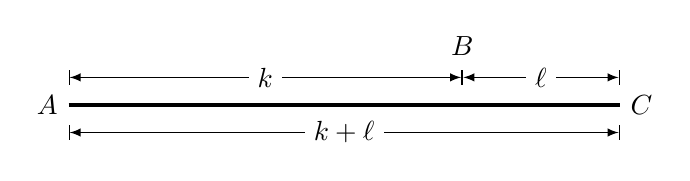
\begin{tikzpicture}[>=latex]
\draw[|<->|] (0,-.35)--node[fill=white]{$k+\ell$}(7,-.35);
\draw[|<->|] (0,.35)--node[fill=white]{$k$}(5,.35);
\draw[|<->|] (5,.35)--node[fill=white]{$\ell$}(7,.35);
\node at (5,.5)[above]{$B$};
\draw[very thick](0,0)node[left]{$A$}--(7,0)node[right]{$C$};

\end{tikzpicture}
    \caption{}\label{fig:length}
\end{figure}

现在我们定义积 $ab$,如\cref{fig:production1},画了一个任意角,在它的一边上,从顶点开始顺次截取长度为 1 和 $b$ 的线段 $OA$ 和 $AC$,在另一边上截取长度为 $a$ 的线段 $OB$,此外,作直线 $CD$ 平行于直线 $AB$,$CD$ 截得的线段 $BD$ 的长度,定义为积 $ab$。这个定义是合理的,因为如果我们在另一个角 $O'$ 上类似地作图(\cref{fig:production2}),那么得到的线段 $B'D'$ 的长度和线段 $BD$ 的长度相等。

\begin{figure}
\begin{minipage}{0.48\linewidth}
  \centering
  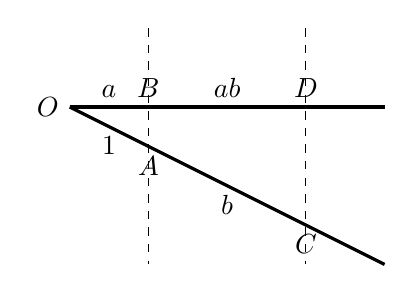
\begin{tikzpicture}
    \draw[very thick] (0,0)node[left]{$O$}--(4,0);
    \draw[very thick] (0,0)--(4,-2);
    \draw[dashed] (1,1)--(1,-2);
    \draw[dashed]  (3,1)--(3,-2);
    \foreach \x/\xtext in {1/B,3/D}
    {
        \node at (\x,0) [above]{$\xtext$};
    }
    \foreach \x/\xtext in {1/A,3/C}
    {
        \node at (\x,-.5*\x) [below]{$\xtext$};
    }
% \node at (2,-2.5){$(1)$};
    \node at (.5,-.25)[below]{1};
    \node at (.5,0)[above]{$a$};
    \node at (2,-1)[below]{$b$};
    \node at (2,0)[above]{$ab$};
  \end{tikzpicture}
  \subcaption{}\label{fig:production1}
\end{minipage}
\begin{minipage}{0.48\linewidth}
  \centering
  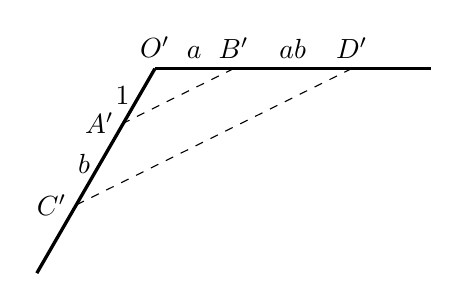
\begin{tikzpicture}
    \draw[very thick] (0,0)node[above]{$O'$}--(3.5,0);
    \draw[very thick] (0,0)--(-120:3);
    \draw[dashed]  (1,0)node[above]{$B'$}--(-120:.8)node[left]{$A'$};
    \draw[dashed]  (2.5,0)node[above]{$D'$}--(-120:2)node[left]{$C'$};
    \node at (.5,0)[above]{$a$};
    \node at (-120:1.4)[left]{$b$};
    \node at (3.5/2,0)[above]{$ab$};
    \node at (-120:.4)[left]{$1$};
  \end{tikzpicture}
  \subcaption{}\label{fig:production2}
\end{minipage}
    \caption{}
\end{figure}

除法运算定义为乘法的逆运算。如\cref{fig:division}, 在角的一边上从顶点开始,顺次截取长度为 $b$ 和 $a$ 的线段,而在另一边上截取单位线段,作 $CD$ 平行于 $AB$, 于是 $AC$ 的长度定义为 $\dfrac{a}{b}$ 这个定义也是合理的,并且 $b\left(\dfrac{a}{b}\right)=a$。

\medskip
最后,我们来规定负长度和零长度。在数轴上,原点 $O$ 右边的点和这点与点 $O$ 的连接线段的长度成一一对应,我们把这种长度称为正的长度。我们把直线上关于原点 $O$ 和点$A$ (即对应长度为 $a$ 的点)对称的点 $A'$ 的相应线段的长度,形式地规定为负的长度 $-a$, 规定点 $O$ 对应于长度零。结果在整个直线上的点和实数之间建立了一一对应。

现在从几何上容易验证实数在四则运算和大小次序这两种结构上满足下面的基本性质,例如,用\cref{fig:distributive_law} 可以验证分配律 $a(b+c)=ab+ac$。

\begin{figure}[htp]
    \begin{minipage}[t]{0.48\textwidth}
    \centering
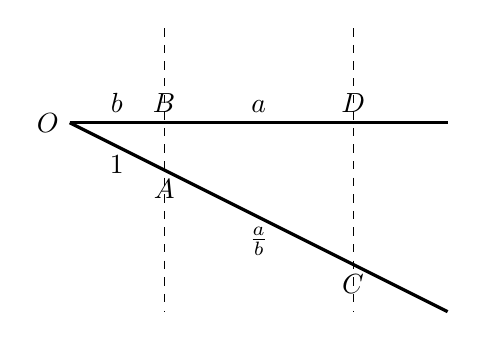
\begin{tikzpicture}[>=latex, scale=1.2]
    \draw[very thick] (0,0)node[left]{$O$}--(4,0);
    \draw[very thick] (0,0)--(4,-2);
    \draw[dashed] (1,1)--(1,-2);
    \draw[dashed]  (3,1)--(3,-2);
    \foreach \x/\xtext in {1/B,3/D}
    {
        \node at (\x,0) [above]{$\xtext$};
    }
    \foreach \x/\xtext in {1/A,3/C}
    {
        \node at (\x,-.5*\x) [below]{$\xtext$};
    }

\node at (.5,-.25)[below]{1};
\node at (.5,0)[above]{$b$};
\node at (2,-1)[below]{$\frac{a}{b}$};
\node at (2,0)[above]{$a$};   
    \end{tikzpicture}
    \caption{}\label{fig:division}
    \end{minipage}
    \begin{minipage}[t]{0.48\textwidth}
    \centering
    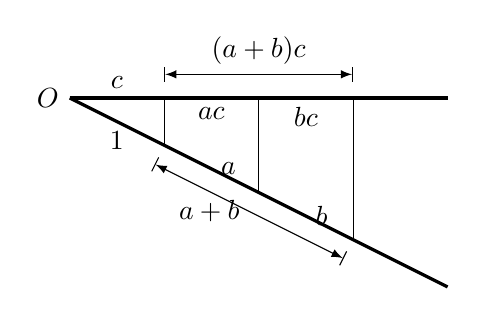
\begin{tikzpicture}[>=latex, scale=1.2]
 \draw[very thick] (0,0)node[left]{$O$}--(4,0);
    \draw[very thick] (0,0)--(4,-2);
    \draw (1,0)--(1,-.5);
    \draw  (2,0)--(2,-1);
    \draw  (3,0)--(3,-1.5);
\node at (.5,-.25)[below]{1};
\node at (.5,0)[above]{$c$};
\node at (1.5,0)[below]{$ac$};   
\node at (2.5,0)[below]{$bc$};   
\node at (1.5,-0.75)[right]{$a$};   
\node at (2.5,-1.25)[right]{$b$};  
\draw[|<->|] (1,.25)--node[above]{$(a+b)c$}(3,.25);
\draw[|<->|] (1-.1,-.5-.2)--node[left]{$a+b$}(3-.1,-1.5-.2);
    \end{tikzpicture}
    \caption{}\label{fig:distributive_law}
    \end{minipage}
    \end{figure}

\subsubsection{加法和乘法的运算性质}

\begin{enumerate}
  \item 交换律:$a+b=b+a;\qquad  ab=ba$
  \item 结合律:$(a+b)+c=a+(b+c);\qquad (a\cdot b)\cdot c=a\cdot (b\cdot c)$
  \item 分配律:$a\cdot (b+c)=a\cdot b+a\cdot c$
  \item 可逆性:$a+x=b;\qquad a\cdot x=b\; (a\ne 0)$ 都是唯一可解的,第一式的解是 $b-a$;第二式的解是 $b/a$。
\end{enumerate}

\subsubsection{顺序性}
\begin{enumerate}
  \item 对于任意实数 $a,b$, 下列关系中有一种且仅有一种成立:
  \[a>b,\qquad a=b\quad \text{或}\quad a<b\]
  \item 由$a<b$和$b<c$推出$a<c$(符号“$<$”的传递性)。
  \item 设$a<b$则$a+c<b+c$
  \item 符号定则
  \[\begin{cases}
      a>0,\qquad b>0\\
      a>0,\qquad b<0\\
      a<0,\qquad b<0
  \end{cases}\Rightarrow\quad  \begin{cases}
      a\cdot b>0\\a\cdot b<0\\a\cdot b>0\\
  \end{cases}\]
  \item 对于任意两个正实数,$a,b>0$, 恒存有一够大的正整数 $n$, 使得 $na<b$。 (通常称之为阿基米德性质)
\end{enumerate}

\subsubsection{ 实数集连续性(完备性)}
我们已经知道实数系与有理数系在加、乘及不等式的运算上有完全相同的性质,但是实数系还具有一个有理数系所没有的优良性质,那就是下面讨论的实数系连续性(完备性)。

在前面,我们用二分法和十分法为例,说明了任何给定的实数 $x$ 都可以用有理数去逼近它。我们所用的是两个有理数列 $\{a_n\}$ 和 $\{b_n\}$ 从左、右夹逼 $x$,$\{a_n\}$,$\{b_n\}$ 和 $x$ 之间的关系可以用下面这一串次序关系来表达:
\[a_1\leqslant a_2\le\cdots\leqslant a_n\leqslant \cdots <x<\cdots\leqslant b_n\leqslant \cdots\leqslant b_2\leqslant b_1\]
$(b_n-a_n)$ 可以任意小,记作 $(b_n-a_n)\to 0$。上面是实数 $x$ 已经先给定了的情况,去求出两串数列 $\{a_n\}$ 和 $\{b_n\}$ 来左、右夹逼实数 $x$,也就是说,数轴$\ell$ 上的每一点,即每一个实数,能够由上述的两个有理数列来唯一确定。反过来问,假如先给定了满足下述这样一串大小次序关系的 $\{a_n\}$ 和 $\{b_n\}$,即
\[a_1\leqslant a_2\le\cdots\leqslant a_n\leqslant \cdots \leqslant b_n\leqslant \cdots\leqslant b_2\leqslant b_1\]
且 $(b_n-a_n)$ 可以任意小,是不是会有那么一个实数 $x$ 去被 $\{a_n\}$、$\{b_n\}$ 左、右夹逼呢?上述问题的答案是肯定的!因为从实数系在长度度量的直观上看,这个实数$x$ 的存在也就是说实数轴上没有空隙存在,即直线是连续不断的,换言之,实数系也是连续不断的,因此我们称实数系为\emph{实数连续统};它说明实数系包含着度量时所有应该包含的数,所以也叫做实数系的\emph{完备性}。下面是直线连续不断的直观概念的解析
描述。

\begin{Theorem}[实数系完备性]{性质}
  对于任给满足下述大小次序关系的两个数列 $\{a_n\}$ 和 $\{b_n\}$,即
\[a_1\leqslant a_2\leqslant \cdots a_n\leqslant \cdots \leqslant b_n\leqslant \cdots \leqslant b_2\leqslant b_1\]
且 $(b_n-a_n)\to 0$,则必定存在一个介于所有 $a_n,b_n$ 之间的实数 $x$。
\end{Theorem}

实数系的完备性是非常基本而且重要的!在以后的章节中,我们将用这个性质来证明极限的存在,从而可进行一切极限运算,而这些运算乃是微积分的基础。在每次用到时,我们将详细解说其用法。这样逐步渐近,同学不难学会它的种种用法。

\begin{Exercise}
\begin{question}
  \item 证明 $\sqrt{3}$ 是无理数。
  \item 设 $\sqrt{5}=a$,$a$ 的小数部分用 $b$ 表示,求 $a-\dfrac{1}{b}$。
  \item 若 $a+\sqrt{b}=c+\sqrt{d}$, 这里 $a,b,c,d$ 是有理数而 $\sqrt{b}$ 是无理数,则 $a=c$,$b=d$,试证之。
  \item 利用“整系数方程 $a_0x^n+a_1x^{n-1}+\cdots+a_{n-1}x+a_n=0$ 的任何有理根,如果写成既约分数时为 $\dfrac{p}{q}$,那么分子 $p$ 是 $a_n$ 的约数,分母 $q$ 是 $a_0$ 的约数”,这一准则使我们能够得到一切有理实根,从而证明任何其它根都是无理数。试证明:$3+2\sqrt{2}$,$1+\sqrt[3]{3}$,$\sqrt[3]{2}+\sqrt[3]{4}$ 都是某一整系数方程的无理根,从而证明这些数都是无理数。
  \item 
  \begin{tasks}
    \task 如果 $a$ 是有理数,$x$ 是无理数,试证明 $a+x$ 是无理数;又如果 $a \neq 0$, 试证明 $ax$ 是无理数。
    \task 试证明任何两个有理数之间至少存在着一个无理数,因而存在着无穷多个无理数。
  \end{tasks}
  \item 试证明:任给无理数 $a$ 和正整数 $m$, 我们可以找到分数 $\dfrac{n}{m}$,使得 \[\left|a-\frac{n}{m}\right|<\frac{1}{2m}\]
  \item 若等腰三角形的顶角为 \ang{36},底边长为 1, 试证它的腰长不能用有理数表示。
  \item 用二分逼近法求下列无理数的有理近似值,使得误差小于 $1/100$:
    \begin{tasks}(2)
        \task $\sqrt{7}$
        \task $\sqrt[3]{2}$
    \end{tasks}
\end{question}
\end{Exercise}

\section{不等式与绝对值}
不等式在高等数学中所起的作用要比在初等数学中大得多,一个量 $x$ 的精确值往往难以确定,不过,对 $x$ 进行估值,即指明 $x$ 大于某个已知量 $a$ 而小于另一个已知量 $b$,却是容易做到的。在许多应用中,重要的只是知道 $x$ 的这种估值。为以后学习方便起见,我们要在这一节比较详细地回顾一下不等式的一些重要性质。

\subsection{不等式的性质}
$a$ 和 $b$ 是实数,如果 $a-b>0$,那么就称 $a$ 大于 $b$,记作 $a>b$;如果 $a-b<0$,那么就称 $a$ 小于 $b$,记作 $a<b$;如果 $a-b=0$ 那么就称 $a$ 等于 $b$,记作 $a=b$。注意若 $a<b$ 有时也说成 $b>a$,因此 $a<b$ 和 $b>a$ 是等价的。

应用两个正实数之和或积仍然是正数这个基本事实,即如果 $a>0$ 和 $b>0$ 则有$a+b>0$ 和 $ab>0$,而且依据不等式 $a>b$ 等价于 $a-b>0$,我们容易推导出下面的性质。

\begin{Theorem}{性质1}
  若 $a>b$ 和 $c>d$,则 $a+c>b+d$。换言之,同向的两个不等式可以相加。
\end{Theorem}

\begin{Theorem}{性质2}
  若 $a>b$ 且 $c>0$,则 $ac>bc$。
\end{Theorem}

\begin{Theorem}{性质3}
  若 $a>b$ 且 $c<0$, 则 $ac<bc$。
\end{Theorem}

上面的性质 2 和性质 3 也可以表达为不等式若乘以正数得到同向不等式;若乘以负数则得到异向的不等式。更一般地可以得到:

若 $a>b>0$ 和 $c>d>0$ 则 $ac>bd$。也就是两个同向的正数不等式可以相乘。
\begin{Theorem}{性质4}
  \begin{itemize}
    \item 若 $a>b>0$, 则 $1/a<  1/b$;
    \item 若 $a>0>b$, 则 $1/a>0>1/b$;
    \item 若 $a<b<0$, 则 $1/a>  1/b$。
  \end{itemize}
\end{Theorem}   

\begin{Theorem}{性质5}
  若 $a>b$ 而 $b>c$, 则 $a>c$。
\end{Theorem}

这就是说不等式具有传递性,在几何上这是显然的,也可由 $(a-b)+(b-c)=a-c$ 为正直接推出,在上述推演中,如果我们处处都用符号 $\geqslant $ 代替 $>$,则各项法则仍然成立。

\begin{Theorem}{性质6}
  若 $a>b>0$, 则 $a^2>b^2$。
\end{Theorem}

我们注意到 $a^2-b^2=(a+b)(a-b)$, 因为 $a+b$ 是正数,由 $a>b$ 可以推出,$a^2>b^2$。这样正数之间不等式可以进行平方运算。

\begin{Theorem}{性质7}
  若 $a>b>0$, 则 $\sqrt{a}>\sqrt{b}$,即在正实数之间的不等式两端能取平方根。
\end{Theorem}

事实上,$\sqrt{a}-\sqrt{b}=\dfrac{a-b}{\sqrt{a}+\sqrt{b}}$,因为 $\sqrt{a}+\sqrt{b}$ 是正数,从而由 $a>b$ 就可推出 $\sqrt{a}-\sqrt{b}>0$, 即$\sqrt{a}>\sqrt{b}$。

更一般地,若 $a>b>0$ 且 $n$ 是自然数,那么 $a^n>b^n$。

这个结论可以用数学归纳法来证明。这个证明留给同学作为练习。

\medskip
反过来,若 $a>b>0$, 且 $n$ 是一个正整数,则 $a^{\frac{1}{n}}>b^{\frac{1}{n}}$。

\begin{proof}
\linespread{1.5}\selectfont
假设 $a^{\frac{1}{n}}=b^{\frac{1}{n}}$,那么$\Big(a^{\tfrac{1}{n}}\Big)^n>\Big(b^{\tfrac{1}{n}}\Big)^n$,因而,$a=b$,这就与已知 $a>b$ 矛盾。

假设 $a^{\frac{1}{n}}<b^{\frac{1}{n}}$,于是 $\Big(a^{\tfrac{1}{n}}\Big)^n<\Big(b^{\tfrac{1}{n}}\Big)^n$,即 $a<b$,这又与已知条件 $a>b>0$ 矛盾,故我们得出结论 $a^{\tfrac{1}{n}}>b^{\tfrac{1}{n}}$。\par
\end{proof}

\subsection{绝对值不等式}
我们回想到$|x|$的定义是这样的:

\begin{Definition}%{定义}
$x$ 是一个实数,当 $x$ 是一个非负数时,$x$ 的绝对值 $|x|$ 是它本身;当 $x$ 是一个负数时,$x$ 的绝对值 $|x|$ 是 $x$ 的相反数。
\begin{equation}
|x|=\begin{cases}
    x,&x\geqslant 0\\
    -x,&x<0
\end{cases}
\end{equation}
\end{Definition}

我们也可以说,当 $x$ 不为零时,$|x|$ 是 $x$ 和 $-x$ 两数之中的较大者;当 $x$ 为零时,$|x|$ 则等于二者之中任何一个。即
\begin{equation}
  \begin{split}
    |x|&=\max\{x,-x\},\qquad (x\ne 0)\\
    |x|&=x=-x,\qquad (x=0)
  \end{split}
\end{equation}

\begin{example}
\[|5|=\max\{5,-5\}=5,\qquad |-5|=\max\{5,-5\}=5,\qquad |0|=0\]
\end{example}

\subsubsection{$|x|$ 的几何意义}
在 $Oxy$ 平面内,$P(x,0)$ 和原点 $O(0,0)$ 之间的距离是
\[d=\sqrt{(x-0)^2+(0-0)^2}=\sqrt{x^2}=|x|\]
因此我们可以说 $|x|$ 是 $P(x,0)$ 点离开原点有 $x$ 单位的\emph{距离}。

\cref{fig:distance} 说明 $|x_2|=|P_2O|$, $|x_1|=|OP_1|$, 其中 $x_2<0$,
$x_1>0$。
\begin{figure}
 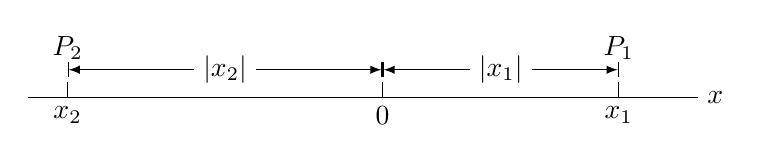
\begin{tikzpicture}[>=latex]
\draw(-.5,0)--(8,0)node[right]{$x$};
\foreach \x/\xtext in {0/x_2,4/0,7/x_1}
{
    \draw (\x,0)node[below]{$\xtext$}--(\x,.2);
}
\draw[|<->|](0,.35)node[above]{$P_2$}--node[fill=white]{$|x_2|$}(4,.35);
\draw[|<->|](7,.35)node[above]{$P_1$}--node[fill=white]{$|x_1|$}(4,.35);

 \end{tikzpicture}
    \caption{}\label{fig:distance}
\end{figure}

如果我们要在 $x$ 轴上描述距离原点不超过 2 个单位的点集,我们把这个条件可以直接写成
\begin{equation}
  \label{eq:abs_neq}
    |x|\leqslant 2
\end{equation}
这个不等式的解集是位于以原点 $O$ 为中心,长度等于 4 的线段上的一切点。\cref{fig:range} 说明这些点的位置。
\begin{figure}
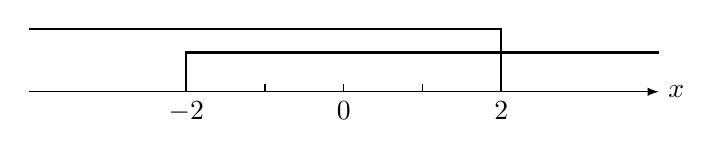
\begin{tikzpicture}[>=latex]
    \draw[->](-4,0)--(4,0)node[right]{$x$};
    \foreach \x in {-2,0,2}
    {
        \draw(\x,0)node[below]{$\x$}--(\x,.1);
    }
    \draw[thick] (-2,0)--(-2,.5)--(4,.5);
    \draw[thick] (2,0)--(2,.8)--(-4,.8);
    \foreach \x in {-1,1}
    {
        \draw(\x,0)--(\x,.1);
    }
\end{tikzpicture}
    \caption{}\label{fig:range} 
\end{figure}

从上面看出这些点的坐标满足不等式
\begin{equation}
  \label{eq:range_neq}
    -2\leqslant x\leqslant 2
\end{equation}
这就是说\cref{eq:abs_neq} 和\cref{eq:range_neq} 是等价的不等式。今后我们将经常遇到的不等式具有下面的形式
\begin{equation}
  \label{eq:abs_neq2}
    |x-a|<3
\end{equation}

$|x-a|=\sqrt{(x-a)^2}$ 的几何意义是 $x$ 轴上的 $P(x,0)$ 点离开 $A(a,0)$ 点的距离。因此已给的不等式是描述在 $x$ 轴上距离 $A(a,0)$ 点小于 3 个单位的点集,根据上面的例题的结论,\cref{eq:abs_neq2} 等价于 $-3<x-a<3$。

不等式的各端加 $a$,得到
\begin{equation}
  a-3<x<a+3    
\end{equation}

因此满足不等式 \eqref{eq:abs_neq2} 的点的坐标是在 $a-3$ 与 $a+3$ 之间(不包括 $a-3$ 和 $a+3$)。

\begin{example}
  在 $x$ 轴上哪些点满足不等式 $|x-3|\leqslant 5$。
\end{example}

\begin{solution}
  $|x-3|\leqslant 5$, 即 $-5\leqslant x-3\leqslant 5$,也即
\[-5+3\leqslant x\leqslant 5+3\]
$\therefore\quad -2\leqslant x\leqslant 8$

这些点位于以 3 为中心,长度等于 10 个单位的线段上,见\cref{fig:solution}。
\begin{figure}
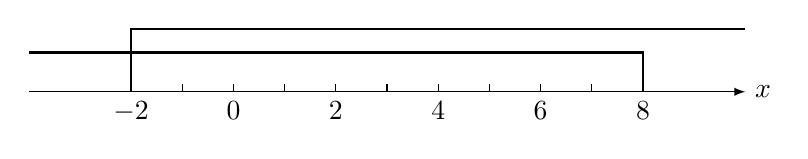
\begin{tikzpicture}[>=latex, xscale=1.3]
    \draw[->](-2,0)--(5,0)node[right]{$x$};
    \foreach \x in {-2,0,2,...,8}
    {
        \draw(\x/2,0)node[below]{$\x$}--(\x/2,.1);
    }
    \foreach \x in {-1,1,...,7}
    {
        \draw(\x/2,0)--(\x/2,.1);
    }
    \draw[thick] (-1,0)--(-1,.8)--(5,.8);
    \draw[thick] (4,0)--(4,.5)--(-2,.5);
\end{tikzpicture}

    \caption{}\label{fig:solution}
\end{figure}

同样地,我们也可以解释 $x>3$ 的几何意义,不等式 $|x|>3$ 是描述在 $x$ 轴上距离原点大于 3 个单位的点集,\cref{fig:solution2} 说明了这些点的位置,图中的圆圈表示去掉 $\pm 3$,因此这些点的坐标小于 $-3$ 或大于 3,即
\[x<-3,\quad \text{或}\quad x>3\]

\begin{figure}
\begin{tikzpicture}[>=latex]
    \draw[->](-4,0)--(4,0)node[right]{$x$};
    \foreach \x in {-3,0,1,3}
    {
        \draw(\x,0)node[below]{$\x$}--(\x,.1);
    }
    \foreach \x in {-2,-1,...,2}
    {
        \draw(\x,0)--(\x,.1);
    }
    \draw[thick] (-3,0)--(-3,.5)--(-4,.5);
    \draw[thick] (3,0)--(3,.5)--(4,.5);
    \foreach \x in {-3,3}
    {
        \draw (\x,0) [fill=white]circle(1.5pt);
    }
\end{tikzpicture}
    \caption{}\label{fig:solution2}
\end{figure}

这就是说,不等式 $|x|>a\; (a>0)$ 等价于不等式 $x<-a$ 或 $x>a\; (a>0)$。
\end{solution}


\begin{example}
  求满足不等式 $(x+2)^2-16>0$ 的点集。
\end{example}

\begin{solution}
  移项
  \[(x+2)^2>16\]
  两边开平方,等价于
  \[|x+2|>4\]
  即
  \[\begin{split}
        x+2<-4\qquad &\text{或}\qquad x+2>4\\  x<-6\qquad &\text{或}\qquad x>2
  \end{split}\]
因此,满足不等式的解集是 $\{x|x<-6\}\cup\{x|x>2\}$。

利用二次函数 $y=(x+2)^2-16$ 的草图,如\cref{fig:parabolic},就更直接地得到 $x<-6$或$x>2$。
\begin{figure}
\begin{tikzpicture}[>=latex, scale=.5]
    \draw[->](-7,0)--(3,0)node[right]{$x$};
    \draw[->](0,-17)--(0,1)node[right]{$y$}; 
\draw[domain=-6.1:2.1, samples=100, thick] plot(\x,{(\x+2)*(\x+2)-16 });
\foreach \y in {-1,-2,...,-16}
{
    \draw (0,\y)--(-.2,\y);
}
\foreach \x in {-6,-5,...,2}
{
    \draw (\x,0)--(\x,.2);
}
\node at (2.5,0)[below]{$2$};
\node at (-6.5,0)[below]{$-6$};
\node at (.5,-.5){$O$};
\node at (0,-16)[right]{$-16$};
\end{tikzpicture}
    \caption{}\label{fig:parabolic}
\end{figure}
\end{solution}

\subsubsection{和、积、商的绝对值}
若 $a$ 和 $b$ 是实数,则 $a\leqslant |a|$ 和 $b\leqslant |b|$,相加得到
\[a+b\leqslant  |a|+|b|\]
同样
\[-a\leqslant |a|\qquad \text{和}\qquad -b\leqslant |b|\]
于是
\[-a-b\leqslant |a|+|b|\]
因为 $a+b$ 和 $-(a+b)$ 都不大于 $|a|+|b|$,所以这两个数中最大者也不大于$|a|+|b|$,于是
\[|a+b|=\max\{a+b,-(a+b)\}\leqslant |a|+|b|\]
这个结果
\begin{equation}
    |a+b|\leqslant |a|+|b|
\end{equation}
常叫做\emph{三角不等式},因为它类似于三角形中任何一边小于其它两边之和这个定理。

有时,我们需要 $|a+b|$ 的下限估值,注意到
\[|a|=|(a+b)-b| \leqslant |a+b| +|-b| =|a+b| +|b|\]
因此下面不等式成立
\begin{equation}
  |a+b|\geqslant |a|-|b|
\end{equation}

若 $a,b$ 是任何实数,则
\[|ab|=\sqrt{(ab)^2}=\sqrt{a^2b^2}=\sqrt{a^2}\cdot \sqrt{b^2}=|a|\cdot |b|\]
即
\begin{equation}
  |ab|=|a|\cdot |b|
\end{equation}
\[\left|\frac{a}{b}\right|=\sqrt{\left(\frac{a}{b}\right)^2}=\sqrt{\frac{a^2}{b^2}}=\frac{\sqrt{a^2}}{\sqrt{b^2}}=\frac{|a|}{|b|}\]
即
\begin{equation}
    \left|\frac{a}{b}\right|=\frac{|a|}{|b|}
\end{equation}


\begin{Exercise}
\begin{question}
  \item 解不等式组:
    \[\begin{cases}
      \dfrac{x}{2}-\dfrac{x}{3}>-1\\
      2(x-3)-3(x-2)<0
    \end{cases}\]
  \item 解不等式:
  \begin{tasks}(2)
      \task $|2x-1|<2|1-2x|-3$
      \task $|x+1|+|x-5|>3$
      \task $\left|\dfrac{3x}{x+1}-3\right|<0.01$
      \task $\dfrac{3x-1}{x-5}<2$
  \end{tasks}
  \item 图示满足下面不等式组的点 $(x,y)$的区域 $R$。
  \[\begin{cases}
      |x-1|+|y-5|<1\\
  y>5+|x-1|
  \end{cases}\]
  \item 试证明若 $ax^2+bx+c>0$ 对于任何 $x$ 都成立的充要条件是 $a>0$ 且 $b^2-4ac<0$。
  \item 等差数列与等比数列的首项相等且第 $2n+1$ 项也相等,问第 $n+1$ 项如何?
  \item 若 $x+2y=1$, 求 $xy$ 的最大值。
  \item 平移 $y=-\dfrac{1}{3}x^2$ 使其顶点在抛物线 $y=x^2$ 上,试求这样得到任何一条抛物线都不能经过的范围,并画图表示。
  \item 求证
  \begin{tasks}
    \task $|a+b+c|\leqslant |a|+|b|+|c|$
    \task $|a-b-c|\geqslant |a|-|b|-|c|$
    \task $\Big| |a|-|b| \Big|\leqslant |a+b|$
  \end{tasks}
  \item \begin{tasks}
    \task 若 $|h|<\frac{\varepsilon}{4}$,$|k|<\frac{\varepsilon}{6}$,求证 $|2h-3k|<\varepsilon$。
    \task 若 $|a_n-r|<\varepsilon$,$|a_n-a_n'|<\varepsilon$,求证 $|a_n'-r|<\varepsilon$。
    \task 若 $|b_n|<\varepsilon$,$|a_n-b_n|<\varepsilon$,求证 $|a_n|<2\varepsilon$。
  \end{tasks}
  \item 试用 $a$ 表出从点 $(0,a)$ 到曲线 $y=\left|\frac{x^2}{2}-1\right|$ 上的点 $(x,y)$ 的距离的最小值 $(a>1)$。
  \item 解不等式 $\sqrt{2x^2-3x-2}>x-1$。
\end{question}
\end{Exercise}

\subsection{几个重要的不等式}
下面我们来推导几个常用的著名不等式。

\begin{example}\label{exp:bernoulli}
  贝努利不等式。若 $n\in\mathbb{N}$且$n\geqslant 2$, $a>-1$ 且 $a \neq 0$(即 $a>0$ 或 $-1<a<0$ ),则
\[(1+a)^n>1+na\]
\end{example}

\begin{proof}
\begin{enumerate}
  \item 对于 $n=2$, 因为 $(1+a)^2=1+2a+a^2$,又 $a^2>0$,故不等式成立。
  \item 假设不等式对于 $n=k$ 成立,即
  \[(1+a)^k>1+ka\]
  我们来证明不等式对于 $n=k+1$ 也成立,就是说
  \[(1+a)^{k+1}>1+(k+1)a\]

  事实上,由假设 $1+a>0$,故不等式
  \[(1+a)^k(1+a)>(1+ka)(1+a)\]
  成立,即
  \[(1+a)^{k+1}>1+(k+1)a+ka^2\]
  将上面不等式右边舍去正项 $ka^2$,就知道
  \[(1+a)^{k+1}>1+(k+1)a\]
  成立,因此命题对于 $n\geqslant 2$ 的自然数成立。
\end{enumerate}
\end{proof}

\begin{example}
  无论多少个正数的几何平均数不大于其算术平均数,即
\[\frac{a_1+a_2+\cdots+a_n}{n}\geqslant \sqrt[n]{a_1a_2\cdots a_n}\]
\end{example}

\begin{proof}
令 $A=\dfrac{a_1+a_2+\cdots+a_n}{n}$,则题意是说,
\begin{equation}
  \label{eq:avg_proof}
  A^n\geqslant a_1a_2\cdots a_n
\end{equation}
当 $a_1=a_2=\cdots= a_n$ 时,则\cref{eq:avg_proof} 显然成立。如果 $a_1,a_2,\ldots,a_n$ 这 $n$ 个数有不相等的,由于
    \[nA=a_1+a_2+\cdots+a_n\]
即:
\[(a_1-A)+(a_2-A)+\cdots+(a_n-A)=0\]
则必有一大于 $A$, 也必有一小于 $A$, 不妨设 $a_1>A>a_2$,于是,$A-a_1<0$,$A-a_2>0$,把 $a_1,a_2,\ldots,a_n$ 改换成
\begin{equation}
  \label{eq:new_series}
a_1'=A,\; a_2'=a_2+a_1-A,\; a_3'=a_3,\; \ldots, a_n'=a_n
\end{equation}
由此可见我们新得之 $n$ 个数,其和不变,即
\[\begin{split}
    a'_1+a'_2+\cdots +a'_n&=A+(a_2+a_1-A)+a_3+\cdots +a_n\\
&= a_1+a_2+\cdots +a_n\\
&=nA
\end{split}\]
但其积增大,因为
\[\begin{split}
    A(a_2+a_1-A)-a_1a_2&=Aa_2+Aa_1-A^2-a_1a_2\\
&=A(a_2-A)+a_1(A-a_2)\\
&=(A-a_2)(a_1-A)>0
\end{split}\]
从而
\[A(a_2+a_1-A)a_3\cdots a_n>a_1a_2\cdots a_n\]
若\cref{eq:new_series} 中还有不等于 $A$ 的,比如,$a_s>A>a_m$,我们用同法即用 $A$ 取代其中较大的一个 $a_c$,用 $a_m+a_s-A$ 代换 $a_m$,又可另得 $n$ 个正数,其和同前,而其积更大。由此以往,不过 $n-1$ 次,便可得 $n$ 个相等之正数$\underbrace{A,A,\cdots A}_{\text{$n$个}}$,此时积最大,故有
\[A^n\geqslant a_1a_2\cdots a_n\]
且当 $a_1=a_2=\cdots =a_n$ 时,等式成立。
\end{proof}

\begin{example}\label{exp:Cauchy}
  柯西不等式,若 $a_i,b_i,\; i=1,2,\cdots ,n$ 是实数,则
\[(a_1b_1+a_2b_2+\cdots +a_nb_n)\leqslant (a_1^2+a_2^2+\cdots +a_n^2)(b_1^2+b_2^2+\cdots+b_n^2)\]
当且仅当
$\dfrac{a_1}{b_1}=\dfrac{a_2}{b_2}=\cdots=\dfrac{a_n}{b_n}$ 时,等式成立。
\end{example}

\begin{proof}
对于任何实数 $t$, 不等式
\begin{equation}
  \label{eq:cauchy_binom}
  (a_1+tb_1)^2+(a_2+tb_2)^2+\cdots +(a_n+tb_n)^2\geqslant 0
\end{equation}
成立,将\cref{eq:cauchy_binom} 的左端改写成按 $t$ 的降幂排列,得
\begin{equation}
  \label{eq:cauchy_binom2}
   ( b^2_1+b^2_2+\cdots +b^2_n)t^2+2(a_1b_1+\cdots +a_nb_n)t+(a^2_1+a_2^2+
+\cdots +a_n^2)\geqslant 0
\end{equation} 
设 $A=a^2_1+\cdots +a_n^2$,$B=a_1b_1+\cdots +a_nb_n$,$C=b^2_1+\cdots +b^2_n$,
于是\cref{eq:cauchy_binom2} 写成 $Ct^2+2Bt+A>0$,其中 $C\geqslant 0$。
\begin{itemize}
  \item 若 $C=0$, 于是 $b_1=b_2=\cdots =b_n=0$,显然,柯西不等式成立。
  \item 若 $C>0$,因而 
  \[C\left(t+\frac{B}{C}\right)^2+\left(A-\frac{B^2}{C}\right)\geqslant 0\]
  对于任意实数 $t$ 成立。故令 $t=-\dfrac{B}{C}$ 代入,得到
  \[A-\frac{B^2}{C}\geqslant 0,\qquad \text{即}\qquad \frac{AC-B^2}{C}\geqslant 0\]
  $\because\quad C>0,\qquad \therefore\quad B^2\leqslant AC$, 即
\[(a_1b_1+\cdots +a_nb_n)^2\leqslant (a^2_1+\cdots +a^2_n)(b^2_1+\cdots +b^2_n)\]
再由\cref{eq:cauchy_binom} 推知当且仅当 $-t=\dfrac{a_1}{b_1}=\dfrac{a_2}{b_2}=\cdots=\dfrac{a_n}{b_n}$ 时,等式成立。
\end{itemize}
\end{proof}

\begin{example}
  设 $a_1,a_2,\ldots,a_n,b_1,b_2,\ldots,b_n$ 是实数,则
\[\sqrt{\sum^n_{i=1}(a_i+b_i)^2}\leqslant \sqrt{\sum^n_{i=1}a^2_i}+\sqrt{\sum^n_{i=1}b^2_i}\]
\end{example}

\begin{proof}
 \[   \sum^n_{i=1}(a_i+b_i)^2=\sum^n_{i=1}a_i^2+2\sum^n_{i=1}a_ib_i+\sum^n_{i=1}b_i^2\]
由\cref{exp:Cauchy} 柯西不等式知
\[\sum^n_{i=1}a_ib_i\le\left|\sum^n_{i=1}a_ib_i\right|\leqslant \sqrt{\sum^n_{i=1}a_i^2}\sqrt{\sum^n_{i=1}b_i^2}\]
因此:
\[\begin{split}
    \sum^n_{i=1}(a_i+b_i)^2&\leqslant \sum^n_{i=1}a_i^2+2\sqrt{\sum^n_{i=1}a_i^2}\sqrt{\sum^n_{i=1}b_i^2}+\sum^n_{i=1}b_i^2\\
    &=\left(\sqrt{\sum^n_{i=1}a^2_i}+\sqrt{\sum^n_{i=1}b^2_i}\right)^2
\end{split}\]
两边开平方,取算术根即得所证。
\end{proof}    

% \section*{习题6.3}
% \addcontentsline{toc}{subsection}{习题6.3}
\begin{Exercise}
\begin{question}
   \item  若 $a,b,c,d$ 是不相等正数,求证:
\begin{tasks}
    \task $\displaystyle \frac{b}{a}+\frac{c}{b}+\frac{d}{c}+\frac{a}{d}>4$
    \task $\displaystyle \frac{b}{\sqrt{a}}+\frac{a}{\sqrt{b}}>\sqrt{a}+\sqrt{b}$
\end{tasks}
   \item  若 $a_1,a_2$ 表示正数,$p,q$ 表示正整数,求证:
\begin{tasks}
    \task $\displaystyle a_1^{p+q}+a_2^{p+q}\geqslant a_1^pa_2^q+a_1^qa_2^q$
    \task $\displaystyle \frac{a_1^{p+q}+a_2^{p+q}}{2}\geqslant \left(\frac{a_1^p+a_2^p}{2}\right)\left(\frac{a_1^q+a_2^q}{2}\right)$
\end{tasks}

\item 用数学归纳法证明:
若 $a_1>0$,$a_2>0$,$n$ 是正整数,则
\[\frac{a_1^n+a_2^n}{2}\geqslant \left(\frac{a_1+a_2}{2}\right)^n\]
\item 求证,当 $n$ 是 1 或不小于 5 的自然数时,总有 $2^n>n^2$。
\item 设 $0<a<1$,$0<x_0<1$,$x_n=a(1-x_{n-1})+(1-a)x_{n-1},\quad (n=1,2,3,\ldots)$,
\begin{tasks}
  \task 用 $a$ 与 $x_0$ 表示 $x_n$;
  \task 证明 $0<x_n<1$。
\end{tasks}

\item 设 $a>2$,给定数列 $\{x_n\}$,其中$x_1=a$,$x_{n+1}=\dfrac{x^2_n}{2(x_n-1)},\quad (n=1,2,3,\ldots)$,
求证:
\begin{tasks}
  \task $x_n>2$,且$\dfrac{x_{n+1}}{x_n}<1$;
  \task 如果 $a<3$,那么 $x_n\leqslant 2+\dfrac{1}{2^{n-1}}$。
\end{tasks}

\item 若长方形的体积是定值,求全面积的最小值。
\item 求证球内接长方体中,以正方体的体积为最大。
\item 求证在周长都为 $2L$ 的所有三角形中,面积最大的必是等边三角形。
\item 若 $a,b,c$ 是正数且 $abc=8$。

求证:$\sqrt{a^2+b^2}+\sqrt{b^2+c^2}+\sqrt{c^2+a^2}\geqslant 6\sqrt{2}$

\item 若$a>0$, $b>0$, 且$a+b=1$, 
求证:\[\left(a+\frac{1}{a}\right)\left(b+\frac{1}{b}\right)\geqslant \frac{25}{4}\]

\item 若 $a+b+c=1$, 且 $a>0$, $b>0$, $c>0$, 求证:
\begin{tasks}
    \task $\displaystyle \left(\frac{1}{a}-1\right)\left(\frac{1}{b}-1\right)\left(\frac{1}{c}-1\right)\geqslant 8$
    \task $\displaystyle \frac{1}{a}+\frac{1}{b}+\frac{1}{c}\geqslant 9$
\end{tasks}

\item 若 $x,y$ 是实数,且 $x^2+y^2\leqslant 1$,
求证:$|x^2+2xy-y^2|\leqslant \sqrt{2}$

\item 对于任何实数,求证:
\[\sqrt{\frac{a_1^2+a_2^2+\cdots+a_n^2}{n}}\geqslant \frac{a_1+a_2+\cdots+a_n}{n}\]
当且仅当诸数相等时,等式成立。
\item $a+b=1$, $a>0$, $b>0$, 求证 $\sqrt{2a+1}+\sqrt{2b+1}\leqslant 2\sqrt{2}$。
\item 求证:
\[\frac{|x_1+x_2|}{|4+x_1^2| |4+x_2^2|}<\frac{1}{8}\]
\item 对于 $n\geqslant 2$ 的自然数 $n$, 证明不等式
\[2^n>1+n\sqrt{2^{n-1}}\]
\item 对于任何正整数 $k\leqslant n$, 求证:
\[1+\frac{k}{n}\leqslant \left(1+\frac{1}{n}\right)^k\leqslant 1+\frac{k}{n}+\frac{k^2}{n^2}\]
\item 已知 $a,b,c,d,e$ 是实数,满足
\[a+b+c+d+e=8,\qquad a^2+b^2+c^2+d^2+e^2=16\]
试确定 $e$ 的最大值。
\item 半径为 1 的圆内接三角形面积等于 $\dfrac{1}{4}$,设此三角形三边长为 $a,b,c$,求证:
\begin{tasks}
  \task $abc=13$;
  \task $\sqrt{a}+\sqrt{b}+\sqrt{c}<\dfrac{1}{a}+\dfrac{1}{b}+\dfrac{1}{c}$。
\end{tasks}

\item 直角三角形斜边长等于10, 内切圆半径为$a$。求何
时内切圆的半径最大,最大值是多少?
\item 若$n>2$, 求证$(n!)^2>n^n$。
\item 有$n$个实数$a_1,a_2,\ldots,a_n$且
$a_1+a_2+\cdots+a_n=n$
\begin{tasks}
  \task 求证:$\sqrt{|a_1|}+\sqrt{|a_2|}+\cdots+\sqrt{|a_n|}\geqslant \sqrt{n}$
  \task 又 $a^2_1+a_2^2+\cdots+a^2_n=n$,求 $a_1,a_2,\ldots,a_n$ 的值。
\end{tasks}

\item 若 $a,b,c$ 是正实数,求证:$\dfrac{c}{a+b}+\dfrac{a}{b+c}+\dfrac{b}{c+a}\geqslant \dfrac{3}{2}$。
\end{question}
\end{Exercise}

